\section{\textbf{\underline{METHODES DE CONSTRUCTION DES MACs}}}
\subsection{\textbf{\underline{CONSTRUCTION A BASE DES BLOCS CHIFFRES}}}

Les blocs chiffrés sont des algorithmes de chiffrement symétrique qui opèrent sur des blocs de données de taille fixe, généralement de 64 ou 128 bits. Ils utilisent une clé secrète pour transformer le bloc de données en un bloc chiffré. Les blocs chiffrés sont utilisés pour assurer la confidentialité des messages, mais ils peuvent aussi servir à construire des MACs. Pour cela, il faut combiner les blocs chiffrés avec un mode opératoire, qui définit comment les blocs du message sont traités et reliés entre eux. Il existe plusieurs modes opératoires possibles, qui ont des propriétés et des performances différentes. Les plus connus sont le CBC-MAC et le C-MAC.

\subsubsection{\textbf{\underline{LE CBC-MAC}}}

CBC MAC est une fonction à base de blocs chiffrés qui utilise le \textbf{mode CBC (Cipher Block Chaining)} pour chiffrer le message avec la clé secrète. Le MAC est le dernier bloc chiffré obtenu par ce mode. Il a été inventé en \textbf{1981} par \textbf{John Black, Phillip Rogaway et Thomas Shrimpton}. Son principe de fonctionnement est le suivant :

\begin{itemize}
    \item [\textbullet] Le message est divisé en blocs de meme taille, par exemple \textbf{128 bits ou 64 bits}, selon la méthode de chiffrement par blocs utilisé. On ajoute du \textbf{paddding} au message pour compléter le dernier bloc.
    \item [\textbullet] On choisit aléatoirement un \textbf{vecteur d'initialisation (IV)}, il doit etre de meme taille que les blocs du message. L'IV n'est pas secret, il peut etre envoyé avec le message et le MAC.
    \item [\textbullet] On chiffre le premier bloc du message avec la clé secrète en utilisant un algorithme de chiffrement par bloc (généralement AES ou DES). On obtient un premier bloc chiffré.
    \item [\textbullet] On effectue une opération XOR entre le premier bloc chiffré et le deuxième bloc du message. Puis on utilise le resultat de cette operation pour chiffrer le deuxieme bloc du message grace a l'algorithme de chiffrement par bloc et de la meme cle k.
    \item [\textbullet] On repète l'opération XOR et le chiffrement pour tous les blocs du message, en utilisant à chaque fois le meme algorithme de chiffrement par blocs. On obtient ainsi une chaine de blocs chiffrés.
    \item [\textbullet] Le MAC est le dernier bloc chiffré de la chaine.
\end{itemize}

\begin{center}
    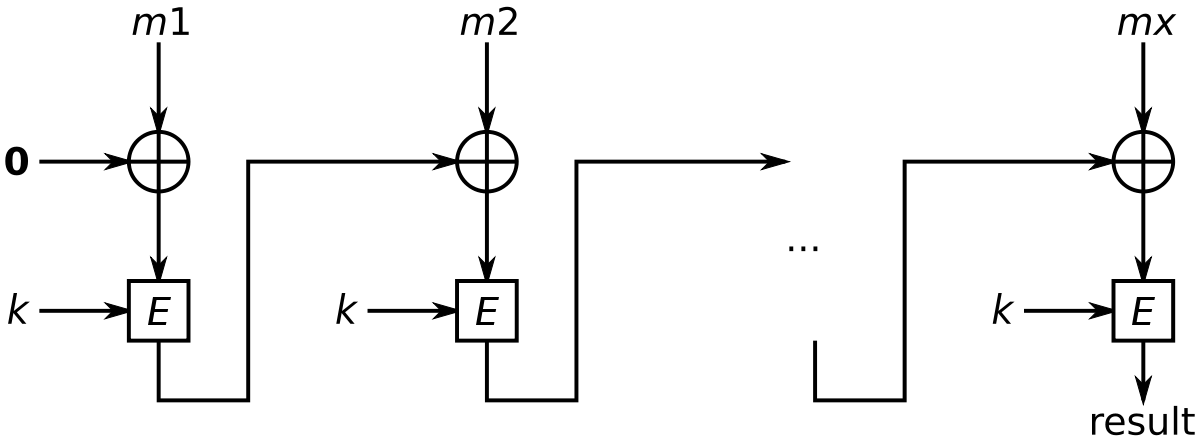
\includegraphics[width=10cm, height=7cm]{Sections/Images/CBC.svg.png}
\end{center}


LE CBC MAC présente tout de meme des failles, les plus connus sont celles de \textbf{l'attaque de Preneel et Van Oorschot, et l'insécurité avec des message de taille vairiable}.\\ 

\textbf{Attaque de Preneel et Van Oordchot}\\

L'attaque décrite par Preneel et Van Oorschot permet de forger des codes d'authentification pour des messages arbitraires sans avoir besoin de connaitre la clé secrète. Pour etre réalisé, l'attaquant a besoin d'environ  $2^{n/2}$ textes connus accompagnés de leurs MACs, forgé avec la clé secrète, où n est la longueur du bloc en bits. L’attaque se déroule comme suit:


\begin{itemize}
    \item [\textbullet] L’attaquant collecte $2^{n/2}$ paires $(M_i, T_i)$, ou $M_i$ est un message de longueur fixe et $T_i$ est son code d’authentification calculé avec le CBC-MAC et la clé secrète k.
    \item [\textbullet] L’attaquant trie les paires selon la valeur de $T_i$ et cherche deux paires $(M_i, T_i)$ et $(M_j, T_j)$ telles que $T_i = T_j$. Il y a une probabilité d’environ $50\%$ qu’il en trouve, selon le paradoxe des anniversaires.
    \item [\textbullet] L’attaquant construit un nouveau message $M = M_i || M_j'$, où $M_j'$ est le message $M_j'$ auquel on a retiré le premier bloc. Le code d’authentification de M est alors $T_j$, car le CBC-MAC de $M_j’$ est égal au CBC-MAC de $M_i$. L’attaquant a donc réussi à forger un code d’authentification sans connaître la clé secrète k.\\
\end{itemize} 

\textbf{Solutions pour renforcer le CBC-MAC}\\

Pour pallier aux limites du CBC-MAC, plusieurs solutions ont été imaginés telles que:

\begin{itemize} 
    \item [\textbullet] Utiliser des clés différentes pour le chiffrement et le code MAC, afin d’éviter les interférences entre les deux opérations
    \item [\textbullet] Utiliser des clés dérivées de la clé principale pour chaque longueur de message possible, afin d’éviter les attaques par concaténation.
    \item [\textbullet] Ajouter un bloc final contenant la longueur du message, afin de distinguer les messages de taille variable.
    \item [\textbullet] Utiliser des variantes du CBC-MAC, comme le CMAC, qui utilise des opérations supplémentaires pour éviter les collisions entre les codes d’authentification.
\end{itemize}
\subsubsection{\textbf{\underline{Le C-MAC}}}

Le \textbf{C-MAC} est une variante du CBC-MAC qui utilise 2 clés secrètes : Une fois le MAC obtenu avec CBC, il suffit de le rechiffrer avec la deuxième clé secrète. Les deux cles sont obtenus en utilisant la cle secrete et une derivation key qui est au prealable passe dans une fonction appelee key derivation function qui permet de dupliquer et d'obtenir deux cles pseudo-aleatoirement.Avec la premiere cle on effectuera le meme procede que celui du CBC MAC et pour chiffrer le deuxieme bloc on utilise la deuxieme cle.

\newpage
\subsection{\textbf{\underline{CONSTRUCTION A BASE DE FONCTIONS DE HACHAGE}}}

Les \textbf{fonctions de hachage} sont des fonctions mathématiques qui transforment un message de taille arbitraire en une valeur fixe, appelée \textbf{empreinte ou digest}.Elles sont aussi utilisés pour calculer les MACs, pour cela on il faut les combiner avec une clé secrète. La méthode de construction des MACs utilisant une fonction de hachage la plus connue est le H-MAC, mais il existe aussi d'autres méthodes comme le N-MAC.

 \subsubsection{\textbf{\underline{Le H-MAC}}}

\textbf{HMAC} (Keyed-Hash Message Authentication Code) est un algorithme cryptographique largement utilisé qui assure l'authentification et l'intégrité des messages et a été proposé en 1997 par \textbf{Bellare}, \textbf{Canetti}, and \textbf{Krawczyk} dans l'article \textbf{"Keying Hash Functions for Message Authentication."}\\\\
Il repose sur le concept d'utilisation \textbf{d'une fonction de hachage cryptographique en combinaison avec une clé secrète pour générer un code d'authentification de message (MAC)}.\\

L'algorithme HMAC peut être défini comme suit :\\
\begin{enumerate}
    \item \textbf{Sélection d’une fonction de Hachage}\\Sélectionnez une fonction de hachage cryptographique appropriée, telle que MD5, SHA-1 ou SHA-256. Le choix de la fonction de hachage dépend du niveau de sécurité souhaité et des exigences spécifiques de l'application.\\
    \item \textbf{Choix d’une clé secrète}\\Choisissez une clé secrète connue uniquement de l'expéditeur et du destinataire. La longueur de la clé doit être adaptée à la fonction de hachage choisie. Une clé plus longue offre une meilleure sécurité mais peut également affecter les performances.\\
    \item \textbf{Calcule du HMAC}\\Pour calculer le HMAC, effectuez les étapes suivantes :\\ 
    \begin{itemize}
        \item [a)] Si la longueur de la clé dépasse la taille de bloc de la fonction de hachage, réduisez la longueur de la clé en la hachant. Si la longueur de la clé est inférieure à la taille de bloc, ajoutez des octets nuls à la clé pour qu'elle corresponde à la taille de bloc.\\
        \item [b)] Effectuez une opération XOR entre la clé et une valeur spécifique appelée "padding interne" (généralement composée d'octets 0x36 répétés).\\
        \item [c)] Hachez le résultat de l'étape b et le message à l'aide de la fonction de hachage choisie.\\
        \item [d)] Effectuez une opération XOR entre la clé et une valeur différente spécifique appelée "padding externe" (généralement composée d'octets 0x5c répétés).\\
        \item [e)] Concaténez le résultat de l'étape d avec le résultat haché de l'étape c.\\
        \item [f)] Hachez le résultat concaténé à l'aide de la fonction de hachage choisie pour obtenir le HMAC final.\\
    \end{itemize}
\end{enumerate}

\begin{center}
    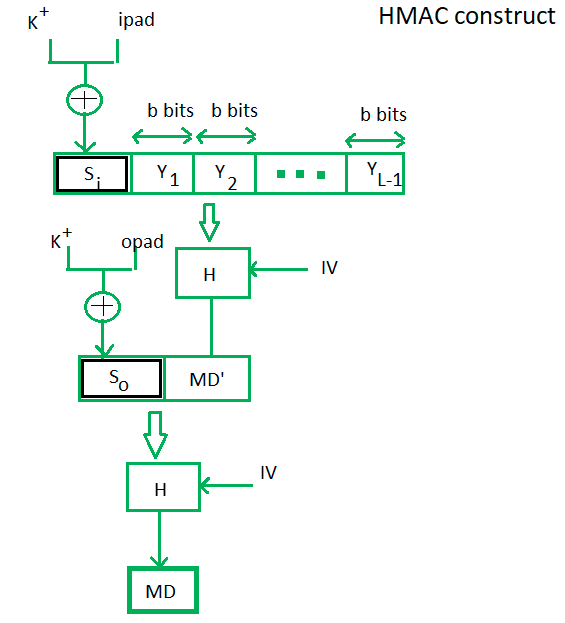
\includegraphics[width=13cm, height=13cm]{Sections/Images/Hash.png}
\end{center}

\newpage
\subsubsection{\textbf{\underline{Le N-MAC}}}

Le \textbf{N-MAC} est une méthode de chiffrement proposé en \textbf{1996} dans un article de \textbf{Mihir Bellare, Ran Conetti et Hugo Krawczyk} dans le but d’améliorer la sécurité du H-MAC, en évitant les attaques basées sue la connaissance partielle de la clé secrète.

\paragraph{Construction du N-MAC}
Le principe de construction du N-MAC est le suivant :
\begin{itemize} 
    \item [\textbullet] On choisit une fonction de hachage H (comme le SHA-256 ou le SHA-512).
    \item [\textbullet] Une clé secrète K.
    \item [\textbullet] On utilise ensuite la fonction de compréssion KDF (key Derivation Function) pour généré les clés K1 et K2 pseudo aléatoirement.
    \item [\textbullet] On calcule S1 = K1 XOR padding interne.
    \item [\textbullet] On calcule S2 = K2 XOR padding externe.
    \item [\textbullet] On calcul le MAC du message M comme :
    MAC (K,K’,M)=H(S1|| H(S2||M) )
\end{itemize}

\paragraph{\textbf{Difficultés}}

Le H-MAC reste tout de même très populaire par rapport au N-MAC car bien que la connaissance partielle de la clé secrète mettrait en danger la sécurité, en pratique, il est très difficile de trouver la \textbf{valeur de la clé secrète interne à partir du MAC}. Même si on connaît le message et la fonction de hachage.
En effet, \textbf{la fonction de hachage est supposée être résistante aux préimages, c’est à dire, qu’il est très difficile de trouver une entrée qui produit une sortie donnée}.Ainsi, pour trouver la clé interne K’, il faudrait résourdre \textbf{l’équation H(K’||M) = MAC}, ce qui est considéré comme infaisable avec les fonctions de Hachage actuelles.De plus, le fait que le N-MAC utilise 2 clés complique la gestion la gestion et la distribution des clés entre les communiquant.

\newpage


\subsection{\textbf{\underline{METHODES DE CONSTRUCTION A BASE DES CODES CORRECTEURS D'ERREURS}}}


Dans le domaine des codes d'authentification de message (MAC), il existe des constructions basées sur des codes correcteurs d'erreurs, technique de codage basee sur la redondance  qui permet non seulement de vérifier l'intégrité des données, mais également de détecter et corriger les éventuelles erreurs de transmission.Les codes correcteurs ont ete invente par Richard Hamming en 1947.Deux constructions couramment utilisées dans les MAC sont le U-MAC et le V-MAC

\subsubsection{\textbf{\underline{ U-MAC (Universal Message Authentication Code)}}}

\textbf{U-MAC} est une construction basée sur les codes correcteurs d'erreurs qui offre à la fois \textbf{l'authentification et la correction d'erreurs}. Il utilise un code correcteur d'erreurs linéaire pour détecter et corriger les erreurs de transmission. Les codes correcteurs d'erreurs linéaires les plus 
couramment utilisés dans le U-MAC sont le \textbf{code de Hamming et le code de Reed-Solomon}.

Voici une description plus détaillée des étapes du U-MAC :
\begin{itemize}[label=$\cdot$]
    \item \textbf{Division du message en blocs :} Le message à authentifier est divisé en blocs de taille fixe. Chaque bloc peut contenir un certain nombre de bits, par exemple 512 bits.
    \item \textbf{Encodage des blocs :} Chaque bloc est encodé à l'aide d'un code correcteur d'erreurs linéaire. L'encodage ajoute des bits de redondance au bloc, ce qui permet de détecter et de corriger les erreurs. Le choix du code correcteur d'erreurs dépend des caractéristiques spécifiques de l'application, telles que le niveau d'erreur attendu et la capacité de correction requise.
    \item \textbf{Génération du MAC :} Une fois les blocs encodés, un MAC est généré pour chaque bloc en utilisant une fonction de hachage cryptographique, telle que SHA-256. Le MAC est calculé sur le bloc encodé, ainsi que sur un numéro de séquence et une clé secrète partagée entre l'expéditeur et le destinataire. Le numéro de séquence est utilisé pour éviter les attaques de rejeu, où un attaquant tente de réutiliser des messages précédemment authentifiés.
    \item \textbf{Transmission des blocs encodés et des MAC }: Les blocs encodés sont transmis avec leurs MAC correspondants. Le destinataire reçoit les blocs encodés et les MAC associés.
    \item \textbf{Vérification du MAC et décodage des blocs :} Le destinataire vérifie l'intégrité des données en recalculant le MAC pour chaque bloc reçu et en le comparant avec le MAC reçu. Si les MAC correspondent, cela indique que le bloc n'a pas été altéré. Ensuite, le destinataire décode les blocs encodés pour récupérer le message d'origine.
    \item \textbf{Correction des erreurs :} Si des erreurs sont détectées dans un bloc, le destinataire utilise les bits de redondance ajoutés lors de l'encodage pour corriger les erreurs. Cela garantit que le message d'origine est récupéré correctement.Le U-MAC offre une combinaison de fonctionnalités d'authentification, de détection et de correction d'erreurs, ce qui en fait une construction robuste pour les applications nécessitant une transmission fiable des données.
\end{itemize} 
\newpage

\subsubsection{\textbf{\underline{Le V-MAC}}}

Le \textbf{V-MAC} est une autre construction basée sur les codes correcteurs d'erreurs, mais avec la particularité de prendre en charge des messages de longueur variable. Contrairement au U-MAC, qui travaille avec des blocs de taille fixe, le V-MAC \textbf{permet d'authentifier des messages de longueur variable, ce qui le rend plus flexible dans certains scénarios.} Il a ete invente par Ted Krovertz et Philip Rogaway


Le V-MAC offre une flexibilité supplémentaire par rapport au U-MAC en \textbf{permettant l'authentification de messages de longueur variable.} Cela peut être utile dans des scénarios où la taille des messages peut varier considérablement, tels que \textbf{les communications en temps réel ou les transferts de fichiers.}\\

Les constructions basées sur les codes correcteurs d'erreurs, comme le U-MAC et le V-MAC, offrent des fonctionnalités d'authentification, de détection et de correction d'erreurs pour assurer l'intégrité des données lors de leur transmission. Ces constructions combinent des codes correcteurs d'erreurs avec des fonctions de hachage cryptographique et des clés secrètes partagées pour garantir la fiabilité des échanges de données. Le choix entre le U-MAC et le V-MAC dépend des exigences spécifiques de l'application et de la nature des messages à authentifier.


\subsection{\textbf{\underline{Référence de cette partie}}}
\begin{center}
    \cite{frwiki:208453934}\\
    \cite{fouque:des-aes}\\
    \cite{frwiki:202365614}\\
    \cite{image:cbc-mac}\\
    \cite{wiki:hash_function}\\
    \cite{okta:hmac}\\
    \cite{okta:umac}\\
    \cite{geeksfg}\\
    \cite{wiki:hmac}\\
    \cite{wiki:umac}\\
    \cite{ionos:hash_function}\\
    \cite{bellare1996new}\\
    \cite{contini2006forgery}\\
    \cite{dodis2012message}
    
\end{center}